\documentclass{beamer}

\usepackage{epsfig}
\usetheme{Boadilla}

\title{Swimming Downstream}
\subtitle{Plans for Topics in GlueX Tracking}
\author[M.\ Ito]{Mark M.\ Ito}
\date{December 7, 2007}
\institute[JLab]{Jefferson Lab}

\newcommand{\bitem}{\begin{itemize}}
\newcommand{\eitem}{\end{itemize}}
\newcommand{\benum}{\begin{enumerate}}
\newcommand{\eenum}{\end{enumerate}}
\newcommand{\bcent}{\begin{center}}
\newcommand{\ecent}{\end{center}}

\newcommand{\Evec}{{\bf E}}
\newcommand{\Bvec}{{\bf B}}
\newcommand{\vvec}{{\bf v}}
\newcommand{\pvec}{{\bf p}}
\newcommand{\kvec}{{\bf k}}
\newcommand{\rvec}{{\bf r}}

\begin{document}

\frame{\titlepage}

\frame{
\frametitle{Overview}
\bitem
\item Overall goal: least-squares track fitting framework
  \bitem
  \item non-uniform magnetic field
  \item geometry independent
  \eitem
\item swimming
\item fitting
\eitem
}

\frame{
\frametitle{choices for swimming}
\bitem
\item    EGS
\item    geant3
\item    geant4
\item   DTrajectory
\item    google
\eitem
}

\frame{
\frametitle{Michel's scheme}

F.~Curtis Michel, ``Numerical integration of trajectories in static magnetic fields,'' http://cnx.org/content/m12765/latest/

Start with Eq.\ (1) of Ref.\ 1.
$$ {\bf F} = e(\Evec + \vvec \times \Bvec) $$
If $\Evec = 0$
$$ {d\pvec \over dt} = e(\vvec \times \Bvec)$$
Also
$$ \pvec = \gamma m \vvec .$$
If we
let $k_1 = e\Delta t / \gamma m$ then
$$ \Delta \vvec = k_1 (\bar\vvec \times \Bvec) $$
where $\Delta \vvec = \vvec^\prime - \vvec$ and $\bar\vvec = (\vvec^\prime + \vvec)/2$.
If we define the vector $\kvec = k_1\Bvec/2$, then
$$ \vvec^\prime = \vvec + [(\vvec^\prime + \vvec) \times \kvec] $$
}
\frame{
the $x$-component of this equation is
$$v_x^\prime = v_x + (v_y^\prime + v_y)k_z - (v_z^\prime + v_z) k_y$$
recovering eq.\ (24) of Ref.\ 1. Rewriting this as
$$ v_x^\prime - v_y^\prime k_z + v_z^\prime k_y = v_x + v_yk_z - v_zk_y $$
we note that all three components in matrix notation can be written as
$$
\begin{pmatrix}
1 & -k_z & k_y \cr
k_z & 1 & -k_x \cr
-k_y & k_x & 1 \cr
\end{pmatrix}
\begin{pmatrix}
v_x^\prime\cr
v_y^\prime\cr
v_z^\prime\cr
\end{pmatrix}
=
\begin{pmatrix}
1 & k_z & -k_y \cr
-k_z & 1 & k_x \cr
k_y & -k_x & 1 \cr
\end{pmatrix}
\begin{pmatrix}
v_x\cr
v_y\cr
v_z\cr
\end{pmatrix}
$$
recovering Eq.\ (25) (without the typo). 
We can write this as
$$
(I+A)\vvec^\prime = (I-A)\vvec
$$
where the anti-symmetric matrix
$$
A=\begin{pmatrix}
0 & -k_z & k_y \cr
k_z & 0 & -k_x \cr
-k_y & k_x & 0 \cr
\end{pmatrix} 
$$
and $I$ is the identity matrix.

} \frame {

Let $M = (I+A)^{-1}(I-A)$ and $\vvec = (\rvec_1 - \rvec_0)/\Delta t$ and $\vvec^\prime = (\rvec_2 - \rvec_1)/\Delta t$. Then we have
$$
\rvec_2 = \rvec_1 + M(\rvec_1 - \rvec_0)
$$
which we can iterate.

comments:

\bitem
\item      more accurate than Rutta-Kunge
\item      simple implementation
\item      time-of-flight info for free
\eitem
}

\frame{
\frametitle{$B = 4$~T, $p = 1$~GeV/$c$, $x$ vs.\ $z$}
$$
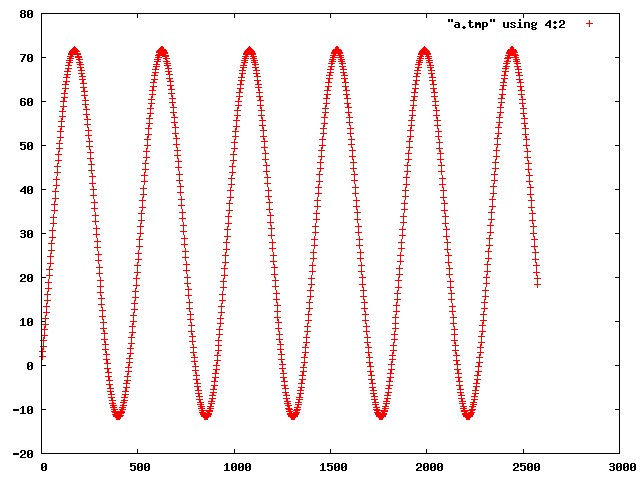
\includegraphics[height=6cm]{xz.jpg}
$$
}

\frame{
\frametitle{$B = 4$~T, $p = 1$~GeV/$c$, $y$ vs.\ $z$}
$$
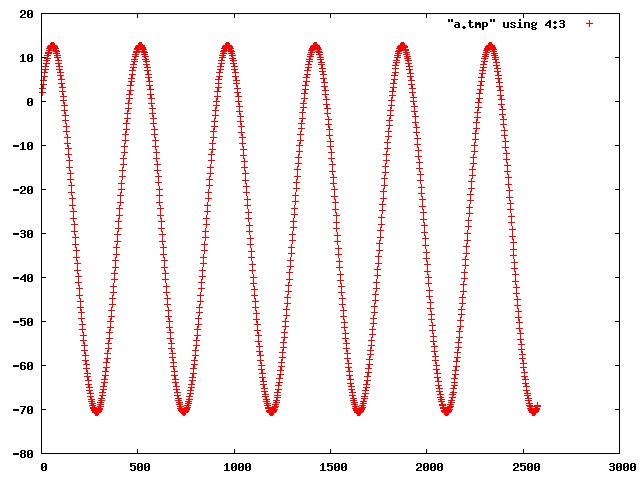
\includegraphics[height=6cm]{yz.jpg}
$$
}

\frame{
\frametitle{$B = 4$~T, $p = 1$~GeV/$c$, $x$ vs.\ $y$}
$$
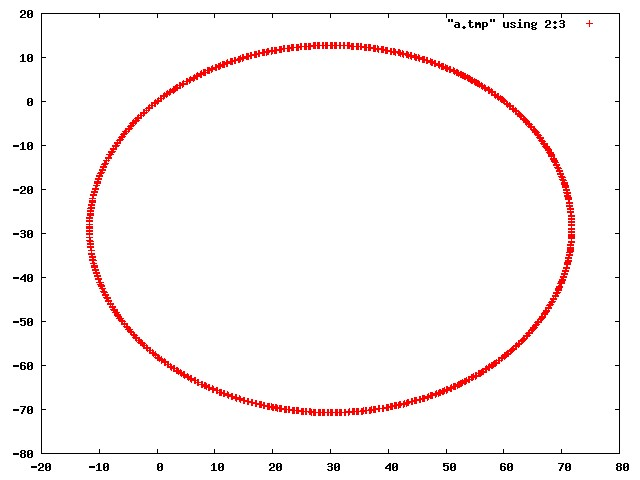
\includegraphics[height=6cm]{xy.jpg}
$$
}

\begin{frame}[fragile]
\frametitle{MyTrajectory C++ class}

base class

\begin{verbatim}
class MyTrajectory {
 public:
  MyTrajectory();
  void swim(HepVector startingPoint,
            double theta, double phi);
  double doca(HepVector& spacePoint);
...
\end{verbatim}

derived class

\begin{verbatim}
class MyTrajectoryHelix : public MyTrajectory {
 public:
  MyTrajectoryHelix(HepVector B);
  void swim(double charge, HepVector startingPoint,
            double p, double theta, double phi);
...
\end{verbatim}

\end{frame}

\frame {
\frametitle{swimming future}
\bitem
\item      B-field map
\item      comparison with others methods
\eitem
}

\frame{

\frametitle{fitting:
  distance of closest approach (DOCA) member function}
\begin{columns}
  \begin{column}[t]{4cm}
\bitem
\item    iterated parabolic interpolation
  \bitem
  \item    independent of functional form
  \eitem
\item    point-to-trajectory done
  \bitem
  \item      good for FDC pseudo-points
  \eitem
\item    line-to-trajectory to do
\eitem
  \end{column}
  \begin{column}[t]{5cm}
    \begin{figure}
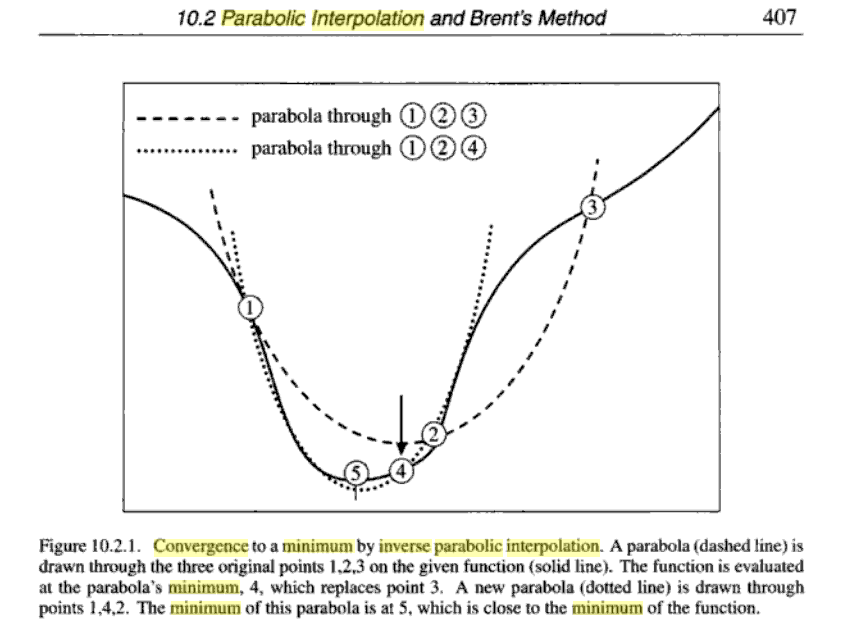
\includegraphics[height=4cm]{para_interp.png}
    \end{figure}
  \end{column}
\end{columns}
}

\frame{
\frametitle{fitting: $\chi^2$ minimizer}
    \bitem
    \item GNU Scientific Library (GSL) non-linear least squares fitter
        \bitem
        \item method name???
        \item weighted or unweighted
        \item depends on (weighted) residuals only
        \item implemented in C
        \eitem
    \item C++ wrapper written, being tested
      \bitem
      \item ugly work around for C++
      \item problem with C callback to C++ member functions
      \item ROOT also has wrapper
      \eitem
    \eitem
}
\frame{
\frametitle{fitting: to do...put pieces together}
\bitem
\item    swimmer
    \item DOCA
    \item GSL $\chi^2$ fitter
\eitem
}

\end{document}

%%% end of latex file %%%%

